% tikz_test.tex
% Comprehensive Test File for TikZ Style Library
% ============================================================
% This file demonstrates all macros and styles defined in tikz_styles.tex
% Compile with: pdflatex tikz_test.tex

\documentclass[11pt,a4paper]{article}

\usepackage[utf8]{inputenc}
\usepackage[T1]{fontenc}
\usepackage{amsmath,amssymb}
\usepackage[margin=1in]{geometry}
\usepackage{booktabs}
\usepackage{array}
\usepackage{float}
\usepackage{multirow}

% Load the TikZ style library
% tikz_styles.tex
% TikZ Style Library for Mobile Anyons from Fusion Categories
% ============================================================
% This file provides a comprehensive collection of TikZ styles and macros
% for drawing fusion category diagrams, including:
%   - Fusion trees and morphism diagrams
%   - F-moves (associators) and pentagon equations
%   - R-moves (braiding) and hexagon equations
%   - Evaluation/coevaluation (cups and caps)
%   - Anyon chains and string diagrams

% ============================================================
% Required TikZ Libraries
% ============================================================
\usepackage{tikz}
\usetikzlibrary{
    positioning,           % Relative positioning
    shapes.geometric,      % Geometric shapes
    decorations.markings,  % Arrow decorations on paths
    decorations.pathmorphing, % Wavy/snake lines
    decorations.pathreplacing, % Braces
    arrows,                % Arrow tips
    arrows.meta,           % Modern arrow tips
    knots,                 % Knot crossings for braiding
    calc,                  % Coordinate calculations
    shapes,                % Additional shapes
    backgrounds,           % Background layers
    fit                    % Fitting nodes
}

% ============================================================
% Color Definitions
% ============================================================
% Primary colors for objects/anyons
\definecolor{AnyonRed}{RGB}{221, 6, 0}
\definecolor{AnyonBlue}{RGB}{15, 105, 197}
\definecolor{AnyonGreen}{RGB}{11, 170, 21}
\definecolor{AnyonOrange}{RGB}{238, 143, 0}

% Gray for boxes and backgrounds
\definecolor{LightGray}{RGB}{220,220,220}
\definecolor{MediumGray}{RGB}{180,180,180}

% ============================================================
% Basic Arrow Styles for String Diagrams
% ============================================================
% Arrow at 60% along the path (standard direction)
\tikzset{->-/.style={
    decoration={markings, mark=at position .6 with {\arrow[>=stealth]{>}}},
    postaction={decorate}
}}

% Arrow at 52% (for certain diagram types)
\tikzset{-->--/.style={
    decoration={markings, mark=at position .52 with {\arrow[>=stealth]{>}}},
    postaction={decorate}
}}

% Reverse arrow at 60%
\tikzset{-<-/.style={
    decoration={markings, mark=at position .6 with {\arrow[>=stealth]{<}}},
    postaction={decorate}
}}

% Arrow at 50% (centered)
\tikzset{->>-/.style={
    decoration={markings, mark=at position .5 with {\arrow[>=stealth]{>}}},
    postaction={decorate}
}}

\tikzset{-<<-/.style={
    decoration={markings, mark=at position .5 with {\arrow[>=stealth]{<}}},
    postaction={decorate}
}}

% Arrow at different positions for longer strands
\tikzset{->>>-/.style={
    decoration={markings, mark=at position .5 with {\arrow[>=stealth]{>}}},
    postaction={decorate}
}}

\tikzset{-<<<-/.style={
    decoration={markings, mark=at position .4 with {\arrow[>=stealth]{<}}},
    postaction={decorate}
}}

% ============================================================
% Morphism Box Styles
% ============================================================
% Standard morphism box (gray rounded rectangle)
\tikzset{morphism box/.style={
    rectangle,
    draw,
    rounded corners,
    fill=LightGray,
    text centered,
    minimum height=0.7cm,
    minimum width=0.9cm,
    font=\small
}}

% Small morphism box
\tikzset{morphism box small/.style={
    morphism box,
    minimum height=0.5cm,
    minimum width=0.6cm,
    font=\scriptsize
}}

% Large morphism box (for composite morphisms)
\tikzset{morphism box large/.style={
    morphism box,
    minimum height=1cm,
    minimum width=1.2cm
}}

% ============================================================
% Fusion Vertex Styles
% ============================================================
% Filled vertex (standard trivalent vertex)
\tikzset{fusion vertex/.style={
    circle,
    fill=black,
    inner sep=1.5pt,
    outer sep=0pt
}}

% Empty vertex (for unfilled vertices)
\tikzset{fusion vertex empty/.style={
    circle,
    draw,
    fill=white,
    inner sep=1.5pt,
    outer sep=0pt
}}

% ============================================================
% Label Styles
% ============================================================
% Object labels (on strands)
\tikzset{object label/.style={
    font=\small,
    fill=white,
    inner sep=1pt
}}

% Vertex labels (multiplicity indices at vertices)
\tikzset{vertex label/.style={
    font=\tiny,
    fill=white,
    inner sep=0.5pt
}}

% Coefficient labels (for F-matrices, R-matrices)
\tikzset{coeff label/.style={
    font=\footnotesize,
    midway,
    fill=white,
    inner sep=1pt
}}

% ============================================================
% Commutative Diagram Arrow Style
% ============================================================
\tikzset{cd arrow/.style={
    ->,
    >=stealth,
    thick
}}

% Pentagon/Hexagon diagram arrow
\tikzset{
    pentagon arrow/.style={
        postaction={decorate},
        decoration={markings, mark=at position 1 with {\arrow[scale=1,thick]{>}}}
    }
}

% ============================================================
% MACROS FOR COMMON DIAGRAMS
% ============================================================

% ------------------------------------------------------------
% Trivalent Vertex (splitting): c -> a tensor b
% Usage: \trivalentvertex{a}{b}{c}
% ------------------------------------------------------------
\newcommand{\trivalentvertex}[3]{%
\begin{tikzpicture}[scale=0.7,baseline={(0,0.2)}]
    \draw (0,0) -- +(90:1) node[above] {\small $#3$};
    \draw (0,0) -- +(225:1) node[below] {\small $#1$};
    \draw (0,0) -- +(315:1) node[below] {\small $#2$};
\end{tikzpicture}%
}

% ------------------------------------------------------------
% Left-associative Fusion Tree: ((a,b)_e, c)_d
% Usage: \fuselefttree{a}{b}{e}{c}{d}
% ------------------------------------------------------------
\newcommand{\fuselefttree}[5]{%
\begin{tikzpicture}[scale=0.425,baseline={(0,0.4)}]
    \draw (0,0) node[below] {\small $#1$} -- (1.5,1.5) -- (3,0) node[below] {\small $#4$};
    \draw (0.75,0.75) -- (1.5,0) node[below] {\small $#2$};
    \draw (0.7,1.6) node {\small $#3$};
    \draw (1.5,1.5) -- (1.5,2.25) node[above] {\small $#5$};
\end{tikzpicture}%
}

% ------------------------------------------------------------
% Right-associative Fusion Tree: (a, (b,c)_e)_d
% Usage: \fuserighttree{a}{b}{e}{c}{d}
% ------------------------------------------------------------
\newcommand{\fuserighttree}[5]{%
\begin{tikzpicture}[scale=0.425,baseline={(0,0.4)}]
    \draw (0,0) node[below] {\small $#1$} -- (1.5,1.5) -- (3,0) node[below] {\small $#4$};
    \draw (2.25,0.75) -- (1.5,0) node[below] {\small $#2$};
    \draw (2.3,1.6) node {\small $#3$};
    \draw (1.5,1.5) -- (1.5,2.25) node[above] {\small $#5$};
\end{tikzpicture}%
}

% ------------------------------------------------------------
% F-move (Associator) Equation
% Displays: left tree = sum_f F * right tree
% Usage: \Fmoveequation{a}{b}{c}{d}{e}{f}
% ------------------------------------------------------------
\newcommand{\Fmoveequation}[6]{%
\begin{tikzpicture}[baseline=(current bounding box.center),scale=0.9]
    % Left tree: ((a b)_e c)_d
    \begin{scope}
        \draw (0,0.5) -- (0,1);
        \draw (0,1) -- (-0.5,1.5);
        \draw (-0.5,1.5) -- (-1,2);
        \draw (-0.5,1.5) -- (0,2);
        \draw (0,1) -- (0.5,1.5);
        \draw (0.5,1.5) -- (1,2);
        \node at (0,0.25) {\small $#4$};
        \node at (-1,2.25) {\small $#1$};
        \node at (0,2.25) {\small $#2$};
        \node at (1,2.25) {\small $#3$};
        \node at (-0.5,1.1) {\small $#5$};
    \end{scope}
    % Equals sign
    \node at (1.8,1.25) {$=\displaystyle\sum_{#6} \left(F_{#4}^{#1#2#3}\right)_{#6#5}$};
    % Right tree: (a (b c)_f)_d
    \begin{scope}[xshift=5.5cm]
        \draw (0,0.5) -- (0,1);
        \draw (0,1) -- (-0.5,1.5);
        \draw (-0.5,1.5) -- (-1,2);
        \draw (0.5,1.5) -- (0,2);
        \draw (0,1) -- (0.5,1.5);
        \draw (0.5,1.5) -- (1,2);
        \node at (0,0.25) {\small $#4$};
        \node at (-1,2.25) {\small $#1$};
        \node at (0,2.25) {\small $#2$};
        \node at (1,2.25) {\small $#3$};
        \node at (0.5,1.1) {\small $#6$};
    \end{scope}
\end{tikzpicture}%
}

% ------------------------------------------------------------
% Evaluation (Cup): X* tensor X -> 1
% Usage: \evalcup{X}
% ------------------------------------------------------------
\newcommand{\evalcup}[1]{%
\begin{tikzpicture}[scale=0.85,baseline=(current bounding box.center)]
    \node at (-0.3,0) {$#1^*$};
    \node at (1.7,0) {$#1$};
    \draw (0,0) arc (180:0:0.7);
\end{tikzpicture}%
}

% ------------------------------------------------------------
% Coevaluation (Cap): 1 -> X tensor X*
% Usage: \coevalcap{X}
% ------------------------------------------------------------
\newcommand{\coevalcap}[1]{%
\begin{tikzpicture}[scale=0.85,baseline=(current bounding box.center)]
    \node at (-0.3,0) {$#1$};
    \node at (1.7,0) {$#1^*$};
    \draw (0,0) arc (-180:0:0.7);
\end{tikzpicture}%
}

% ------------------------------------------------------------
% Left Zigzag Identity (Snake equation)
% Usage: \leftzigzag{X}
% ------------------------------------------------------------
\newcommand{\leftzigzag}[1]{%
\begin{tikzpicture}[baseline=(current bounding box.center)]
    \draw (0,0) -- (0,1);
    \draw (0,1) arc (0:180:0.4);
    \draw (-0.8,1) arc (0:-180:0.4);
    \draw (-1.6,1) -- (-1.6,2);
    \node at (0.25,0) {$#1$};
    \node at (-1.85,2) {$#1$};
    \node at (-1.05,1) {$#1^*$};
\end{tikzpicture}%
}

% ------------------------------------------------------------
% Right Zigzag Identity (Snake equation)
% Usage: \rightzigzag{X}
% ------------------------------------------------------------
\newcommand{\rightzigzag}[1]{%
\begin{tikzpicture}[baseline=(current bounding box.center)]
    \draw (0,0) -- (0,1);
    \draw (0,1) arc (180:0:0.4);
    \draw (0.8,1) arc (-180:0:0.4);
    \draw (1.6,1) -- (1.6,2);
    \node at (-0.25,0) {$#1^*$};
    \node at (1.85,2) {$#1^*$};
    \node at (1.05,1) {$#1$};
\end{tikzpicture}%
}

% ------------------------------------------------------------
% Simple Braiding (Over-crossing): X crosses over Y
% Usage: \braidingover{X}{Y}
% ------------------------------------------------------------
\newcommand{\braidingover}[2]{%
\begin{tikzpicture}[scale=0.85,baseline=(current bounding box.center)]
    \node at (-0.75,0.35) {$#1$};
    \node at (-0.75,2.65) {$#2$};
    \node at (0.75,0.35) {$#2$};
    \node at (0.75,2.65) {$#1$};
    \draw (-0.4,0.2) -- (-0.4,0.5);
    \draw (-0.4,2.5) -- (-0.4,2.8);
    \draw (0.4,0.2) -- (0.4,0.5);
    \draw (0.4,2.5) -- (0.4,2.8);
    \begin{knot}[flip crossing/.list={8},consider self intersections=true,ignore endpoint intersections=false]
        \strand (-0.4,0.5)to[out=90,in=270](0.4,2.5);
        \strand (0.4,0.5)to[out=90,in=270](-0.4,2.5);
    \end{knot}
\end{tikzpicture}%
}

% ------------------------------------------------------------
% Inverse Braiding (Under-crossing): X crosses under Y
% Usage: \braidingunder{X}{Y}
% ------------------------------------------------------------
\newcommand{\braidingunder}[2]{%
\begin{tikzpicture}[scale=0.85,baseline=(current bounding box.center)]
    \node at (-0.75,0.35) {$#2$};
    \node at (-0.75,2.65) {$#1$};
    \node at (0.75,0.35) {$#1$};
    \node at (0.75,2.65) {$#2$};
    \draw (-0.4,0.2) -- (-0.4,0.5);
    \draw (-0.4,2.5) -- (-0.4,2.8);
    \draw (0.4,0.2) -- (0.4,0.5);
    \draw (0.4,2.5) -- (0.4,2.8);
    \begin{knot}[flip crossing/.list={8},consider self intersections=true,ignore endpoint intersections=false]
        \strand (0.4,0.5)to[out=90,in=270](-0.4,2.5);
        \strand (-0.4,0.5)to[out=90,in=270](0.4,2.5);
    \end{knot}
\end{tikzpicture}%
}

% ------------------------------------------------------------
% Twist (Ribbon element): curl on a single strand
% Usage: \twist{X}
% ------------------------------------------------------------
\newcommand{\twist}[1]{%
\begin{tikzpicture}[scale=1.1,baseline=(current bounding box.center)]
    \node at (1,0.7)[left] {$#1$};
    \begin{knot}[flip crossing/.list={4,5},consider self intersections=true,ignore endpoint intersections=false]
        \strand (1,0.5)--(1,1);
        \strand (1,1)to[out=90,in=180](1.25,1.75)to[out=0,in=90](1.45,1.5)to[out=270,in=0](1.25,1.25)to[out=180,in=270](1,2);
        \strand (1,2)--(1,2.5);
    \end{knot}
\end{tikzpicture}%
}

% ------------------------------------------------------------
% Bigon (Bubble): a,b fuse to c then split back
% Usage: \bigon{a}{b}{c}
% ------------------------------------------------------------
\newcommand{\bigon}[3]{%
\begin{tikzpicture}[baseline=(current bounding box.center)]
    \draw (0,0) -- (0,0.5);
    \draw (0,0.5) to[bend left=60] node[left] {$#1$} (0,1.5);
    \draw (0,0.5) to[bend right=60] node[right] {$#2$} (0,1.5);
    \draw (0,1.5) -- (0,2);
    \node at (0,-0.25) {$#3$};
    \node at (0,2.25) {$#3$};
\end{tikzpicture}%
}

% ------------------------------------------------------------
% Quantum Dimension Loop: closed loop labeled X
% Usage: \qdimloop{X}
% ------------------------------------------------------------
\newcommand{\qdimloop}[1]{%
\begin{tikzpicture}[baseline=(current bounding box.center)]
    \draw (0,0) circle (0.5cm);
    \node at (0.75,0) {$#1$};
\end{tikzpicture}%
}

% ------------------------------------------------------------
% Identity Strand: straight vertical line
% Usage: \identitystrand{X}
% ------------------------------------------------------------
\newcommand{\identitystrand}[1]{%
\begin{tikzpicture}[baseline=(current bounding box.center)]
    \draw (0,0) -- (0,2);
    \node at (-0.25,0) {$#1$};
    \node at (-0.25,2) {\phantom{$#1$}};
\end{tikzpicture}%
}

% ------------------------------------------------------------
% Anyon Chain Segment: N anyons with fusion labels
% Usage: Place manually or use as template
% ------------------------------------------------------------
\newcommand{\anyonchain}[1]{%
% Draws a simple anyon chain with sites labeled #1
% Customize as needed for specific applications
\begin{tikzpicture}[scale=1.5,baseline=(current bounding box.center)]
    \node at (0,0) {\textbullet};
    \node at (1,0) {\textbullet};
    \node at (2,0) {\textbullet};
    \node at (3,0) {$\cdots$};
    \draw (0.15,0) -- (0.85,0);
    \draw (1.15,0) -- (1.85,0);
    \draw (2.15,0) -- (2.85,0);
    \node at (0,+0.35) {\small $#1_1$};
    \node at (1,+0.35) {\small $#1_2$};
    \node at (2,+0.35) {\small $#1_3$};
\end{tikzpicture}%
}

% ------------------------------------------------------------
% Splitting Tree: General N-particle splitting
% Usage: Manual construction using standard TikZ
% Template provided as example
% ------------------------------------------------------------
% Example usage for 4-particle splitting tree:
% \begin{tikzpicture}[scale=0.8]
%     \draw (0,0) -- (0,0.5);
%     \draw (0,0.5) -- (-0.5,1);
%     \draw (0,0.5) -- (0.5,1);
%     \draw (-0.5,1) -- (-1,1.5);
%     \draw (-0.5,1) -- (0,1.5);
%     \draw (0.5,1) -- (0.5,1.5);
%     \node at (0,-0.25) {$u$};
%     \node at (-1,1.75) {$a$};
%     \node at (0,1.75) {$b$};
%     \node at (0.5,1.75) {$c$};
%     \node at (-0.55,0.7) {\small $e$};
% \end{tikzpicture}

% ============================================================
% Circled Numbers (for numbered items in diagrams)
% ============================================================
\newcommand{\circlednum}[1]{%
\begin{tikzpicture}[baseline={([yshift=-3pt]current bounding box.center)}]
    \node[circle,scale=0.6,draw] at (0,0) {$#1$};
\end{tikzpicture}%
}

\newcommand{\circlednumcolor}[2]{%
\begin{tikzpicture}[baseline={([yshift=-3pt]current bounding box.center)}]
    \node[circle,scale=0.6,draw=#1] at (0,0) {$#2$};
\end{tikzpicture}%
}

% ============================================================
% Diamond Labels (for F-symbol indices)
% ============================================================
\newcommand{\Fdiamond}[1]{%
\begin{tikzpicture}[baseline={([yshift=-3pt]current bounding box.center)},scale=1]
    \node[diamond,scale=0.35,draw,black] at (0,0) {\huge $#1$};
\end{tikzpicture}%
}

% ============================================================
% Temperley-Lieb Patterns
% ============================================================
% Two parallel arcs (TL identity)
\newcommand{\TLidentity}{%
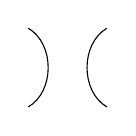
\begin{tikzpicture}[baseline={([yshift=-3pt]current bounding box.center)}]
    \draw (0,0) to [bend right=60] (0,1);
    \draw (1,0) to [bend left=60] (1,1);
\end{tikzpicture}%
}

% Cup-cap pair (TL e_i generator)
\newcommand{\TLcupcap}{%
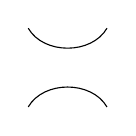
\begin{tikzpicture}[baseline={([yshift=-3pt]current bounding box.center)}]
    \draw (0,0) to [bend left=60] (1,0);
    \draw (0,1) to [bend right=60] (1,1);
\end{tikzpicture}%
}

% H pattern (horizontal connection)
\newcommand{\TLhorizontal}{%
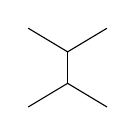
\begin{tikzpicture}[baseline={([yshift=-3pt]current bounding box.center)}]
    \draw (0,0) to (0.5,0.3) to (1,0);
    \draw (0,1) to (0.5,0.7) to (1,1);
    \draw (0.5,0.3) to (0.5,0.7);
\end{tikzpicture}%
}

% ============================================================
% Environment for Full Pentagon Diagram
% ============================================================
% Use the standalone file tex/figures/src/pentagon.tex for the full diagram
% or include inline with the patterns established above.

% ============================================================
% Environment for Full Hexagon Diagram
% ============================================================
% Use the standalone file tex/figures/src/hexagon.tex for the full diagram
% The hexagon.tex in literature/tex provides comprehensive examples.

% ============================================================
% END OF TIKZ STYLE LIBRARY
% ============================================================


\title{TikZ Style Library Test\\
\large Fusion Category Diagrams for Mobile Anyons}
\author{Test Document}
\date{\today}

\begin{document}

\maketitle
\tableofcontents
\newpage

% ============================================================
\section{Basic Fusion Category Diagrams}
% ============================================================

\subsection{Trivalent Vertices}

The basic trivalent vertex represents fusion/splitting:

\begin{center}
\begin{tabular}{ccc}
$\trivalentvertex{a}{b}{c}$ &
$\trivalentvertex{X}{Y}{Z}$ &
$\trivalentvertex{\tau}{\tau}{\tau}$ \\[0.5cm]
\verb|\trivalentvertex{a}{b}{c}| &
\verb|\trivalentvertex{X}{Y}{Z}| &
\verb|\trivalentvertex{\tau}{\tau}{\tau}|
\end{tabular}
\end{center}

\subsection{Fusion Trees}

Left-associative and right-associative fusion trees:

\begin{center}
\begin{tabular}{cc}
$\fuselefttree{a}{b}{e}{c}{d}$ & $\fuserighttree{a}{b}{f}{c}{d}$ \\[0.5cm]
\verb|\fuselefttree{a}{b}{e}{c}{d}| & \verb|\fuserighttree{a}{b}{f}{c}{d}|
\end{tabular}
\end{center}

\subsection{F-Move (Associator)}

The F-move relates different fusion orders:

\[
\Fmoveequation{a}{b}{c}{d}{e}{f}
\]

\begin{center}
\verb|\Fmoveequation{a}{b}{c}{d}{e}{f}|
\end{center}

\subsection{F-Move with Multiplicity Indices}

For categories with $N^c_{ab} > 1$, vertices carry multiplicity labels $\mu, \nu$:

\[
\Fmovemult{a}{b}{c}{d}{e}{f}{\mu}{\nu}
\]

\begin{center}
\verb|\Fmovemult{a}{b}{c}{d}{e}{f}{\mu}{\nu}|
\end{center}

Individual trees with multiplicities for inline use:

\begin{center}
\begin{tabular}{cc}
$\Ftreeleft{a}{b}{c}{d}{e}{\mu}{\nu}$ & $\Ftreeright{a}{b}{c}{d}{f}{\mu'}{\nu'}$ \\[0.5cm]
\verb|\Ftreeleft{a}{b}{c}{d}{e}{\mu}{\nu}| & \verb|\Ftreeright{a}{b}{c}{d}{f}{\mu'}{\nu'}|
\end{tabular}
\end{center}

% ============================================================
\section{Duality: Cups and Caps}
% ============================================================

\subsection{Evaluation and Coevaluation}

\begin{center}
\begin{tabular}{cc}
\textbf{Evaluation (Cup)} & \textbf{Coevaluation (Cap)} \\[0.3cm]
$\evalcup{X}$ & $\coevalcap{X}$ \\[0.3cm]
\verb|\evalcup{X}| & \verb|\coevalcap{X}|
\end{tabular}
\end{center}

\subsection{Zigzag Identities (Snake Equations)}

The zigzag identities express that cups and caps are inverse:

\begin{center}
\begin{tabular}{cc}
$\leftzigzag{X}\ =\ \identitystrand{X}$ &
$\rightzigzag{X}\ =\ \identitystrand{X^*}$ \\[0.5cm]
\verb|\leftzigzag{X}| & \verb|\rightzigzag{X}|
\end{tabular}
\end{center}

\subsection{Bigon and Quantum Dimension}

\begin{center}
\begin{tabular}{ccc}
$\bigon{a}{b}{c}$ & $\qdimloop{X}$ & $\identitystrand{X}$ \\[0.5cm]
\verb|\bigon{a}{b}{c}| & \verb|\qdimloop{X}| & \verb|\identitystrand{X}|
\end{tabular}
\end{center}

% ============================================================
\section{Braiding and R-Moves}
% ============================================================

\subsection{Braiding Crossings}

Over-crossing (positive) and under-crossing (negative):

\begin{center}
\begin{tabular}{cc}
\textbf{Over-crossing} $c_{X,Y}$ & \textbf{Under-crossing} $c_{X,Y}^{-1}$ \\[0.3cm]
$\braidingover{X}{Y}$ & $\braidingunder{X}{Y}$ \\[0.3cm]
\verb|\braidingover{X}{Y}| & \verb|\braidingunder{X}{Y}|
\end{tabular}
\end{center}

\subsection{Twist (Ribbon Element)}

The twist encodes the topological spin:

\begin{center}
$\twist{X}$
\qquad
\verb|\twist{X}|
\end{center}

% ============================================================
\section{Temperley-Lieb Patterns}
% ============================================================

The Temperley-Lieb algebra generators for 2 strands:

\begin{center}
\begin{tabular}{ccc}
\textbf{Identity} & \textbf{Cup-Cap} $(e_i)$ & \textbf{H-pattern} \\[0.3cm]
$\TLidentity$ & $\TLcupcap$ & $\TLhorizontal$ \\[0.3cm]
\verb|\TLidentity| & \verb|\TLcupcap| & \verb|\TLhorizontal|
\end{tabular}
\end{center}

% ============================================================
\section{Trivalent Category Relations}
% ============================================================

For categories generated by a rotationally invariant trivalent vertex with parameters $(d, b, t)$.

\subsection{Loop Relation}

A closed loop evaluates to the quantum dimension $d$:

\begin{center}
$\trivloopeq$
\qquad\qquad
\verb|\trivloopeq|
\end{center}

Or just the loop: $\trivloop$ = \verb|\trivloop|

\subsection{Lollipop (Forbidden Diagram)}

In trivalent categories, lollipops vanish:

\begin{center}
$\trivlollipop\ = 0$
\qquad\qquad
\verb|\trivlollipop|
\end{center}

\subsection{Bigon Relation}

The bigon simplifies to $b$ times the identity:

\begin{center}
$\trivbigoneq$
\end{center}
\begin{center}
\verb|\trivbigoneq|
\end{center}

\subsection{Triangle Relation}

A triangle with external legs equals $t$ times the trivalent vertex:

\begin{center}
$\trivtriangleeq$
\end{center}
\begin{center}
\verb|\trivtriangleeq|
\end{center}

\subsection{Square Diagram}

The square face with four external legs:

\begin{center}
$\trivsquare$
\qquad\qquad
\verb|\trivsquare|
\end{center}

% ============================================================
\section{$\mathfrak{C}_4$ Basis Diagrams}
% ============================================================

In a cubic trivalent category, these four diagrams form a basis for $\mathrm{Hom}(\mathbf{1}, X^{\otimes 4})$:

\begin{center}
\begin{tabular}{cccc}
$w_1$ & $w_2$ & $w_3$ & $w_4$ \\[0.3cm]
$\Cfourone$ & $\Cfourtwo$ & $\Cfourthree$ & $\Cfourfour$ \\[0.5cm]
\verb|\Cfourone| & \verb|\Cfourtwo| & \verb|\Cfourthree| & \verb|\Cfourfour|
\end{tabular}
\end{center}

\subsection{Square Decomposition}

The square decomposes as a linear combination of basis elements:

\[
\trivsquaredecomp
\]

where $\alpha = \frac{b(b^2+bt-t^2)}{bd+t+dt}$ and $\beta = \frac{t^2(d+1)-b^2}{bd+t+dt}$.

% ============================================================
\section{$\mathfrak{C}_5$ Basis Diagrams}
% ============================================================

Representative patterns for 5 boundary points:

\begin{center}
\begin{tabular}{ccc}
\textbf{Star} & \textbf{Chain} & \textbf{Pentagon} \\[0.3cm]
$\Cfivestar$ & $\Cfivechain$ & $\Cfivepentagon$ \\[0.5cm]
\verb|\Cfivestar| & \verb|\Cfivechain| & \verb|\Cfivepentagon|
\end{tabular}
\end{center}

% ============================================================
\section{$\mathfrak{C}_6$ Basis Diagrams}
% ============================================================

Representative patterns for 6 boundary points:

\begin{center}
\begin{tabular}{cccc}
\textbf{Three Bigons} & \textbf{Dumbbell} & \textbf{Hexagon} & \textbf{Pentafork} \\[0.3cm]
$\Csixthreebigon$ & $\Csixdumbbell$ & $\Csixhexagon$ & $\Csixpentafork$ \\[0.5cm]
\verb|\Csixthreebigon| & \verb|\Csixdumbbell| & \verb|\Csixhexagon| & \verb|\Csixpentafork|
\end{tabular}
\end{center}

% ============================================================
\section{Inner Product Pairing}
% ============================================================

The bilinear inner product of two trivalent graphs $f, g$ with $n$ boundary points:

\begin{center}
$\langle f, g \rangle = \trivinnerprod{f}{g}$
\end{center}

\begin{center}
\verb|\trivinnerprod{f}{g}|
\end{center}

% ============================================================
\section{2-Local Hamiltonian Diagrams}
% ============================================================

These diagrams are useful for constructing nearest-neighbor Hamiltonians on anyon chains.

\subsection{Basic 2-Site Operators}

\begin{center}
\begin{tabular}{cccccc}
\textbf{Identity} & \textbf{Swap} & \textbf{Cup-Cap} & \textbf{H-pattern} & \textbf{Braid} & \textbf{Braid$^{-1}$} \\[0.3cm]
$\Htwoidentity$ & $\Htwoswap$ & $\Htwocupcap$ & $\HtwoH$ & $\Htwobraid$ & $\Htwobraidinv$ \\[0.5cm]
\verb|\Htwoidentity| & \verb|\Htwoswap| & \verb|\Htwocupcap| & \verb|\HtwoH| & \verb|\Htwobraid| & \verb|\Htwobraidinv|
\end{tabular}
\end{center}

\subsection{Hopping Operators (Braid with Vacuum)}

Hop operators have one strand as vacuum (dashed) representing anyon hopping:

\begin{center}
\begin{tabular}{cccc}
\textbf{Hop Right} & \textbf{Hop Left} & \textbf{Hop Right$^{-1}$} & \textbf{Hop Left$^{-1}$} \\[0.3cm]
$\Htwohopright$ & $\Htwohopleft$ & $\Htwohoprghtinv$ & $\Htwohopleftinv$ \\[0.5cm]
\verb|\Htwohopright| & \verb|\Htwohopleft| & \verb|\Htwohoprghtinv| & \verb|\Htwohopleftinv|
\end{tabular}
\end{center}

Example hopping Hamiltonian:
\[
H_{\text{hop}} = -t \sum_i \left( \Htwohopright + \Htwohopleft \right)_i
\]

\subsection{Fusion with Intermediate Channel}

\begin{center}
\begin{tabular}{ccc}
$\Htwofusion{c}$ & $\Htwofusion{\mathbf{1}}$ & $\Htwofusion{X}$ \\[0.5cm]
\verb|\Htwofusion{c}| & \verb|\Htwofusion{\mathbf{1}}| & \verb|\Htwofusion{X}|
\end{tabular}
\end{center}

\subsection{Local Operator in Chain Context}

\begin{center}
$\chainlocal{H}$
\qquad\qquad
\verb|\chainlocal{H}|
\end{center}

% ============================================================
\section{Anyon Chain}
% ============================================================

Anyons live in \textbf{intervals} (between lattice sites), not at vertices. Vertical tick marks indicate lattice sites:

\subsection{Standard Chain (with tick marks)}

\begin{center}
$\anyonchain{a}$
\end{center}

\begin{center}
\verb|\anyonchain{a}|
\end{center}

\subsection{Shaded Chain (intervals highlighted)}

\begin{center}
$\anyonchainshaded{\tau}$
\end{center}

\begin{center}
\verb|\anyonchainshaded{\tau}|
\end{center}

% ============================================================
\section{Utility Macros}
% ============================================================

\subsection{Circled Numbers}

\begin{center}
\begin{tabular}{ccccc}
$\circlednum{1}$ & $\circlednum{2}$ & $\circlednum{3}$ & $\circlednumcolor{red}{4}$ & $\circlednumcolor{blue}{5}$ \\[0.3cm]
\verb|\circlednum{1}| & \verb|\circlednum{2}| & \verb|\circlednum{3}| & \verb|\circlednumcolor{red}{4}| & \verb|\circlednumcolor{blue}{5}|
\end{tabular}
\end{center}

\subsection{F-Symbol Diamond}

For labeling F-symbol indices: $\Fdiamond{\alpha}$, $\Fdiamond{\beta}$

\begin{center}
\verb|\Fdiamond{\alpha}|, \verb|\Fdiamond{\beta}|
\end{center}

% ============================================================
\section{Compact Braiding for Hamiltonians}
% ============================================================

Compact (squatter) braids for use inside brackets:

\begin{center}
\begin{tabular}{cccc}
\textbf{Compact} & \textbf{Compact Inv} & \textbf{Labeled} & \textbf{Labeled Inv} \\[0.3cm]
$\braidcompact$ & $\braidcompactinv$ & $\braidlabeled{a}{b}$ & $\braidlabeledinv{a}{b}$ \\[0.5cm]
\verb|\braidcompact| & \verb|\braidcompactinv| & \verb|\braidlabeled{a}{b}| & \verb|\braidlabeledinv{a}{b}|
\end{tabular}
\end{center}

Example in a Hamiltonian expression:
\[
H = -\sum_i \left( \braidcompact + \phi^{-1}\, \braidcompactinv \right)_i
\]

% ============================================================
\section{Color Definitions}
% ============================================================

Professional complementary color scheme (blue-orange with accents):

\begin{center}
\begin{tabular}{lll}
\textbf{Name} & \textbf{Sample} & \textbf{Usage} \\[0.2cm]
\hline\\[-0.2cm]
AnyonBlue & \textcolor{AnyonBlue}{\rule{1cm}{0.4cm}} & Primary color \\
AnyonOrange & \textcolor{AnyonOrange}{\rule{1cm}{0.4cm}} & Complementary color \\
AnyonTeal & \textcolor{AnyonTeal}{\rule{1cm}{0.4cm}} & Accent color \\
AnyonCoral & \textcolor{AnyonCoral}{\rule{1cm}{0.4cm}} & Accent color \\
AnyonSlate & \textcolor{AnyonSlate}{\rule{1cm}{0.4cm}} & Dark emphasis \\
AnyonSilver & \textcolor{AnyonSilver}{\rule{1cm}{0.4cm}} & Subtle elements \\
LightGray & \textcolor{LightGray}{\rule{1cm}{0.4cm}} & Backgrounds \\
MediumGray & \textcolor{MediumGray}{\rule{1cm}{0.4cm}} & Borders \\
\end{tabular}
\end{center}

% ============================================================
\section{TikZ Styles Reference}
% ============================================================

\subsection{Arrow Styles}

\begin{center}
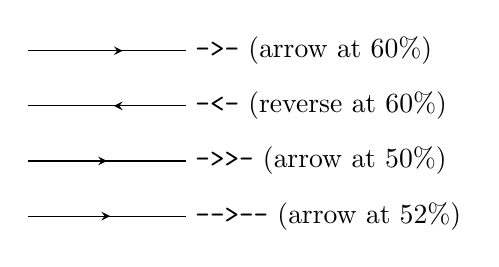
\begin{tikzpicture}
    \draw[->-] (0,0) -- (2,0) node[right] {\texttt{->-} (arrow at 60\%)};
    \draw[-<-] (0,-0.7) -- (2,-0.7) node[right] {\texttt{-<-} (reverse at 60\%)};
    \draw[->>-] (0,-1.4) -- (2,-1.4) node[right] {\texttt{->>-} (arrow at 50\%)};
    \draw[-->--] (0,-2.1) -- (2,-2.1) node[right] {\texttt{-->--} (arrow at 52\%)};
\end{tikzpicture}
\end{center}

\subsection{Box and Vertex Styles}

\begin{center}
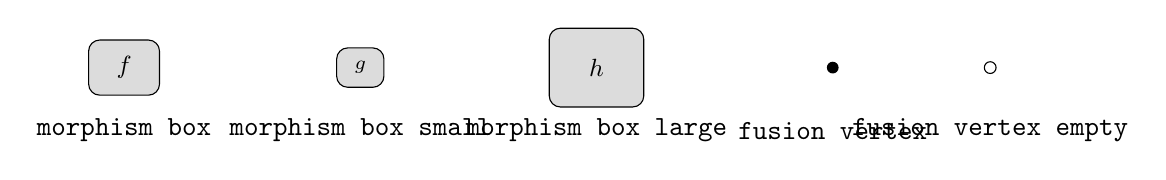
\begin{tikzpicture}
    \node[morphism box] at (0,0) {$f$};
    \node at (0,-0.8) {\texttt{morphism box}};

    \node[morphism box small] at (3,0) {$g$};
    \node at (3,-0.8) {\texttt{morphism box small}};

    \node[morphism box large] at (6,0) {$h$};
    \node at (6,-0.8) {\texttt{morphism box large}};

    \node[fusion vertex] at (9,0) {};
    \node at (9,-0.8) {\texttt{fusion vertex}};

    \node[fusion vertex empty] at (11,0) {};
    \node at (11,-0.8) {\texttt{fusion vertex empty}};
\end{tikzpicture}
\end{center}

% ============================================================
\section{Example: Golden Chain Hamiltonian}
% ============================================================

As an example, here is how to write a 2-local Hamiltonian term for the golden chain using these macros (note proper vertical centering in brackets):

\[
H = -\sum_i \left( \Htwofusion{\mathbf{1}} + \phi^{-1} \Htwofusion{\tau} \right)_i
\]

where $\phi = \frac{1+\sqrt{5}}{2}$ is the golden ratio.

The projector onto the trivial fusion channel at sites $i, i+1$ is:

\[
P^{(\mathbf{1})}_{i,i+1} = \frac{1}{d} \Htwocupcap
\]

All 2-local operators side by side for comparison:
\[
\left( \Htwoidentity \right) \quad
\left( \Htwoswap \right) \quad
\left( \Htwocupcap \right) \quad
\left( \HtwoH \right) \quad
\left( \Htwofusion{c} \right) \quad
\left( \Htwobraid \right) \quad
\left( \Htwobraidinv \right)
\]

% ============================================================
\section{Example: Trivalent Category Calculation}
% ============================================================

In the Fibonacci category with $d = \phi$, $b = 1$, $t = \frac{d-2}{d-1}$:

\[
\trivloop = d = \phi \approx 1.618
\]

\[
\trivbigon = b \cdot \begin{tikzpicture}[scale=0.7,baseline=(current bounding box.center)]
    \draw (0,0) -- (0,1.2);
\end{tikzpicture} = 1 \cdot \begin{tikzpicture}[scale=0.7,baseline=(current bounding box.center)]
    \draw (0,0) -- (0,1.2);
\end{tikzpicture}
\]

The four basis diagrams in $\mathfrak{C}_4$ satisfy:

\[
\Cfourfour - \Cfourthree + \frac{1}{d+1}\Cfourone + \frac{1}{d-1}\Cfourtwo = 0
\]

% ============================================================
\appendix
\section{Quick Reference Card}
% ============================================================

\begin{table}[H]
\centering
\small
\begin{tabular}{lll}
\toprule
\textbf{Category} & \textbf{Macro} & \textbf{Output} \\
\midrule
\multirow{3}{*}{Vertices}
& \verb|\trivalentvertex{a}{b}{c}| & $\trivalentvertex{a}{b}{c}$ \\
& \verb|\fuselefttree{a}{b}{e}{c}{d}| & $\fuselefttree{a}{b}{e}{c}{d}$ \\
& \verb|\fuserighttree{a}{b}{f}{c}{d}| & $\fuserighttree{a}{b}{f}{c}{d}$ \\
\midrule
\multirow{2}{*}{Duality}
& \verb|\evalcup{X}| & $\evalcup{X}$ \\
& \verb|\coevalcap{X}| & $\coevalcap{X}$ \\
\midrule
\multirow{3}{*}{Braiding}
& \verb|\braidingover{X}{Y}| & $\braidingover{X}{Y}$ \\
& \verb|\braidingunder{X}{Y}| & $\braidingunder{X}{Y}$ \\
& \verb|\twist{X}| & $\twist{X}$ \\
\midrule
\multirow{4}{*}{Trivalent}
& \verb|\trivloop| & $\trivloop$ \\
& \verb|\trivbigon| & $\trivbigon$ \\
& \verb|\trivtriangle| & $\trivtriangle$ \\
& \verb|\trivsquare| & $\trivsquare$ \\
\midrule
\multirow{4}{*}{$\mathfrak{C}_4$ Basis}
& \verb|\Cfourone| & $\Cfourone$ \\
& \verb|\Cfourtwo| & $\Cfourtwo$ \\
& \verb|\Cfourthree| & $\Cfourthree$ \\
& \verb|\Cfourfour| & $\Cfourfour$ \\
\midrule
\multirow{4}{*}{2-Local}
& \verb|\Htwoidentity| & $\Htwoidentity$ \\
& \verb|\Htwocupcap| & $\Htwocupcap$ \\
& \verb|\HtwoH| & $\HtwoH$ \\
& \verb|\Htwofusion{c}| & $\Htwofusion{c}$ \\
\bottomrule
\end{tabular}
\caption{Quick reference for commonly used TikZ macros}
\end{table}

\end{document}
